\documentclass[%
a4paper,
twoside,
12pt
]{article}

% encoding, font, language
\usepackage[T1]{fontenc}
\usepackage[utf8]{inputenc}
\usepackage{lmodern}
\usepackage[ngerman]{babel}

\usepackage{nicefrac}
\usepackage{textcomp}
\usepackage{setspace}

\usepackage[
%    handwritten,
    nowarnings,
    %myconfig
]
{config/xcookybooky}



\DeclareRobustCommand{\textcelcius}{\ensuremath{^{\circ}\mathrm{C}}}


\setcounter{secnumdepth}{1}
\renewcommand*{\recipesection}[2][]
{%
    \subsection[#1]{#2}
}
\renewcommand{\subsectionmark}[1]
{% no implementation to display the section name instead
}


\usepackage{hyperref}    % must be the last package
\hypersetup{%
    pdfauthor            = {Kathrin Welzel and Marcel Gro{\ss}mann},
    pdftitle             = {Wedding Recipes},
    pdfsubject           = {Recipes},
    pdfkeywords          = {wedding, recipes, cookbook},
    pdfstartview         = {FitV},
    pdfview              = {FitH},
    pdfpagemode          = {UseNone}, % Options; UseNone, UseOutlines
    bookmarksopen        = {true},
    pdfpagetransition    = {Glitter},
    colorlinks           = {true},
    linkcolor            = {black},
    urlcolor             = {blue},
    citecolor            = {black},
    filecolor            = {black},
}

\hbadness=10000	% Ignore underfull boxes

\begin{document}
\title{Kochbuch anl"asslich der Hochzeit}
\author{Kathrin Welzel \& Marcel Gro{\ss}mann}

\begin{titlepage}
		\setstretch{1.5}
	\centering\fontsize{80pt}{80pt}\fontfamily{pbk}\selectfont

	Kochbuch
	
	\huge
	anl"asslich der Hochzeit
	
	von
	
	\fontsize{40pt}{40pt}\selectfont
	Kathrin \& Marcel
	
	\vfill
	\begin{figure}[h]
		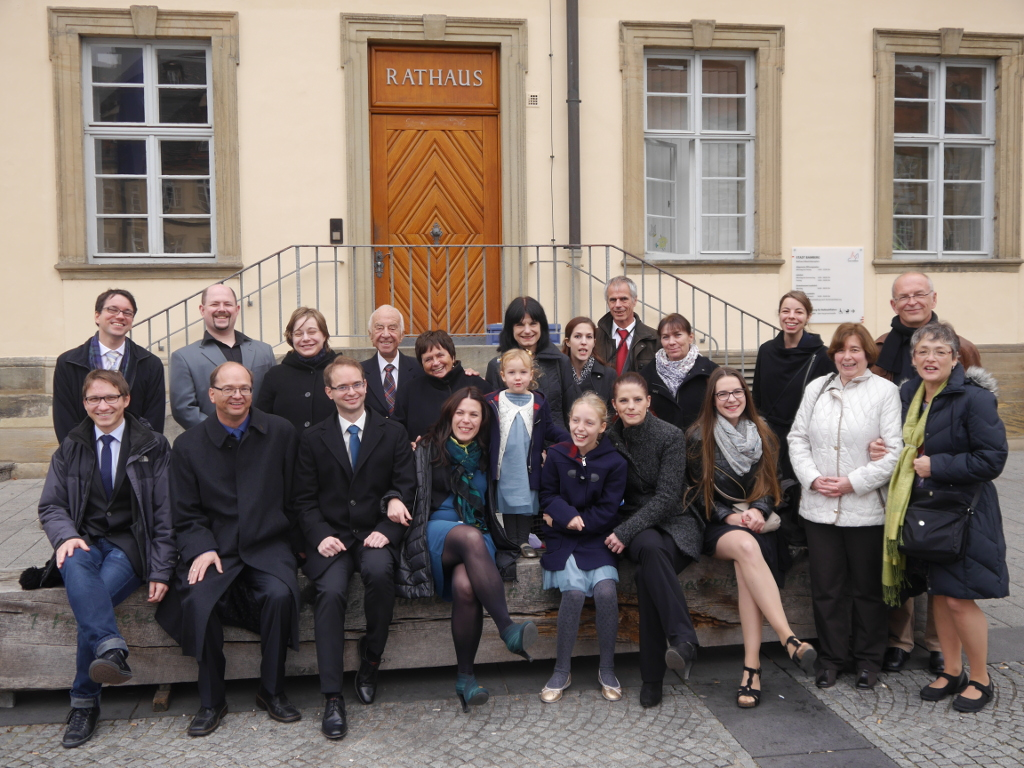
\includegraphics[width=\textwidth]{pic/front.jpg}
	\end{figure}
\LARGE
	\today
\end{titlepage}
\thispagestyle{empty}



\cleardoublepage
\tableofcontents


\cleardoublepage


% background graphic
%\setBackgroundPicture[x, y=-2cm, width=\paperwidth-4cm, height, orientation = pagecenter]{pic/background}

\begin{otherlanguage}{ngerman}
\setHeadlines
{% translation
    inghead = Zutaten,
    prephead = Zubereitung,
    hinthead = Tipp,
    continuationhead = Fortsetzung,
    continuationfoot = Fortsetzung auf n\"achster Seite,
    portionvalue = Personen,
}

%%%%%%%%%%%%%%%%%%%%%%%%%%%%%%%%%%%%%%%%%%%%%%%%%%%%%%%%%%%%%%%%%%%
%				Recipe Section										%
%%%%%%%%%%%%%%%%%%%%%%%%%%%%%%%%%%%%%%%%%%%%%%%%%%%%%%%%%%%%%%%%%%%
\cleardoublepage
\section{Vegetarische Speisen}
\begin{figure}[h]
	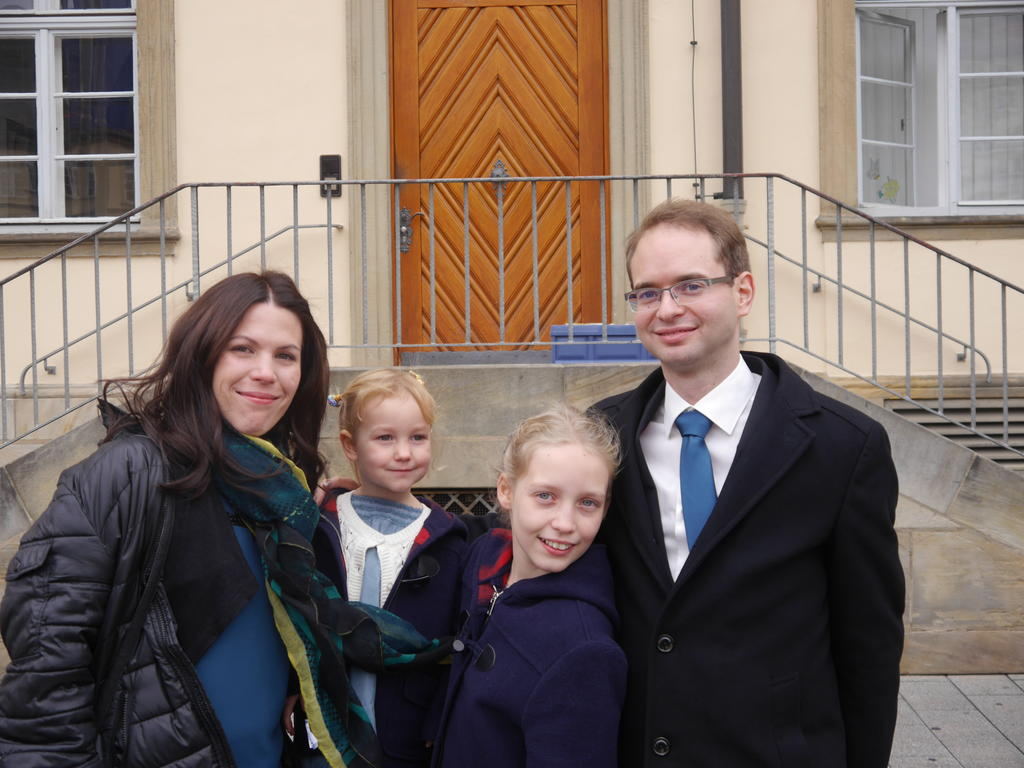
\includegraphics[width=\textwidth]{pic/veggie.jpg}
\end{figure}


\begin{recipe}
[% 
    preparationtime = {\unit[30]{min}},
    portion = {\portion{4}},
    source = {Lieblingsrezept von Ariane (original von chefkoch.de)}
]
{Ratatouille mit Tofu}

    \ingredients{%
        500 g	& 	Tomaten \\
		500 g	& 	Zucchini \\
		500 g &	Paprikaschoten \\
		500 g	&	Aubergine\\
		2	&	Zwiebeln \\
		2	&	Knoblauchzehen \\
		400 g & Räuchertofu \\
		4 EL & Olivenöl\\
		 & Salz und Pfeffer\\
		 2 Stiele & Thymian\\
		2 Stiele & Rosmarin\\
		2 Stiele & Oregano\\
		2 & Lorbeerblatt\\
    }
    
    \preparation{%
    \newline
       \step Das Gemüse gründlich waschen, die Tomaten häuten und in grobe Stücke schneiden. Die Zwiebeln schälen und wie das restliche Gemüse würfeln (ca. erbsengroß). Den Knoblauch schälen und fein hacken. 
       \step Das Olivenöl in einem weiten Topf erhitzen, die Gemüse darin getrennt nach Sorten jeweils 10 Minuten garen, dann herausnehmen (das Gemüse für das Ratatouille getrennt anbraten und erst ganz am Ende miteinander vermischen).
       \step Anschließend den Tofu kurz abtrocknen und würfeln. Das Gemüse vermengen. Die Kräuter mit dem Lorbeerblatt, dem Knoblauch und dem gewürfelten Tofu dazugeben. Mit Salz und Pfeffer würzen und alles weitere 10 Minuten garen.
    }
   
\end{recipe}
% Complete recipe example
\begin{recipe}
% My favourite childhood receipe from my Grandma :)
[%
    preparationtime = {\unit[10]{min}},
    bakingtime={\unit[20]{min}},
    portion = {16--20 pancakes},
    %calory={\unit[3]{kJ}},
    source = {David's favorite Scottish childhood recipe}
]
{Scotch Pancakes (Drop Scones)}

    %\graph
    %{% pictures
        % Unfortunatly I don't have my own picture, but there is an excellent one here: https://www.nigella.com/recipes/scotch-pancakes
    %}

    \ingredients{%
        150 g	         & plain flour \\
                         & pinch of salt \\
        \unitfrac{1}{2} level teasp. & bicarbonate of soda \\
        1 level teasp.   & cream of tartar \\
        1 tablesp.       & caster sugar \\
        1                & beaten egg \\
        1 teasp.         & golden syrup (optional) \\
        120 ml           & milk \\
    }

    \preparation{%
    \newline
       \step Sieve dry ingredients into bowl. Add egg and syrup to mixture. Slowly add milk and beat well to create a batter which will pour from a spoon but must not be too thin. Don't leave standing too long before use.
       \step Heat a heavy frying pan and grease it with lard or white flora. Pour batter on, 1 table spoon at a time (= 1 pancake). Make several at a time but not too close together. When bubbles appear on the surface and just start to burst, turn pancakes over with a palette knife. Cook about 1 minute longer until golden brown.
    }

    \suggestion[Servierbeispiel]
    {%
        Serve with butter and jam.
    }

\end{recipe}

\begin{recipe}
[% 
    preparationtime = {\unit[45]{min}},
    portion = {\portion{2}},
    source = {Ein weiterer Klassiker aus Martins \& Linus' Kochstudio, adaptiert von Chefkoch},
]
{Linus' \& Martins Risotto}
        
    \ingredients{%
		300g	&	Risottoreis\\
		1		& 	Schalotte, klein geschnitten\\
		1 \unitfrac{1}{2} l &	Gem"usebrühe\\
		40g		&	Butter\\
		150ml	&	Weißwein\\
		1 Dose	&	Safranfäden\\
		50g		&	Butter, kalt\\
		150g	&	Parmesan, frisch gerieben\\
				&	Salz\\
				&	Pfeffer
    }
    
    \preparation{%
    \newline
    \step Die Brühe wird in einem Topf heiß gehalten, ohne zu kochen und dann folgt der 1. Schritt, das Anschwitzen -- \textit{solfriggere}. Die Schalotte wird ganz sanft, ohne zu bräunen in 5 Minuten in der Butter angeschwitzt. 
    
    \step Für die 2. Stufe wird der Reis zugegeben und so oft gewendet, bis jedes Korn von der Butter benetzt ist. Dieser Vorgang nennt sich \textit{tostare}. Jetzt wird die Temperatur nach Fingerspitzengefühl leicht erhöht und der Wein angegossen, der ganz verdampfen muss. Nun fügt man den Safran zu. 
    
    \step Schon ist man in der 3. Stufe, dem eigentlichen Kochen, dem \textit{cuocere}, in dem kellenweise die heiße Brühe zugegeben wird. Dieser Vorgang dauert 17 -- 18 Minuten, um einen bissfesten und cremigen Risotto zu kochen. Dabei sollte permanent umgerührt und die Körner vom Rand und Boden des Topfes geschabt werden. 
    
	Die Temperatur muss die Brühe gerade eben kochen lassen und konstant bleiben. Ist die Brühe fast eingekocht, wird die nächste Kelle angegossen. Ab der 14. Minute muss man aufpassen, nicht mehr zu viel Brühe anzugießen, damit der Reis zum Schluss nicht zu flüssig ist. Am Ende des Kochens wird die Hitze deutlich reduziert, um den Reis für 1 Minute ruhen zu lassen. 
    
    \step Dann folgt der 4. und letzte Schritt, die \textit{Mantecatura}, das Verrühren mit kalten Butterwürfeln und frisch geriebenem Parmesan. Nicht vergessen, mit Salz und Pfeffer abzuschmecken. Jetzt sollte die perfekte Konsistenz erreicht sein, die man \textit{Risotto all´onda} nennt. Das bedeutet, wenn man den Topf zur Seite kippt, schlägt der Reis Wellen. 
       
    }
    
    \suggestion[Servierbeispiel]
    {%
		Den Risotto in tiefen Tellern servieren und möglichst bald essen, sonst verliert er seine Konsistenz. Traditionell wird Risotto aber immer ohne Beilagen und erst recht nicht selbst als Beilage gereicht.
    }
    

    \hint{%
       Mehr K"ase ist mehr!
    }
    
\end{recipe}
% Complete recipe example
\begin{recipe}
[% 
    preparationtime = {\unit[65]{min}},
    bakingtime={\unit[20]{min}},
    bakingtemperature={\protect\bakingtemperature{
        topbottomheat=\unit[200]{°C},
       gasstove=Stufe 3}},
    portion = {\portion{4}},
    source = {Lieblingsrezept von Heike und Sarah}
]
{Gratinierter Spargel}
    
    
    \ingredients{%
    &\textbf{Für den Teig:} \\
        100 g	& 	Mehl \\
		\unitfrac{1}{4} Liter	& 	Milch \\
		2 &	Eier (Größe M) \\
			& \textbf{Für die Füllung:}\\
		1 kg	&	Spargel \\
		6 & Tomaten\\
		 \unitfrac{1}{2} Bund & Oregano\\
		 1 & Zwiebel\\
		5 EL & Olivenöl\\
		2-3 EL& Balsamessig\\
		1 Prise & Zucker\\
		& \textbf{Für die Sauce:}\\
		2 EL & Butter\\
		1 geh. EL & Mehl\\
		250 ml & Gemüsebrühe\\
		250 ml & Schlagsahne\\
		& \textbf{Außerdem:}\\
					&	Salz\\
			&	Muskatnuss \\
					&Pfeffer\\
		100 g & geriebener Parmesankäse\\
		60 g & Pinienkerne\\
    }
    
    \preparation{%
    \newline
       \step Mehl mit Milch und Eiern zu einem glatten Teig verquirlen, mit Salz und Muskat würzen. Zugedeckt beiseite stellen.
       \step Spargel waschen, die Enden abschneiden. Spargel in kochendem Salzwasser 6-8 Minuten garen, abtropfen lassen. Tomaten überbrühen, häuten, halbieren und entkernen. Fruchtfleisch fein würfeln. Oregano waschen, trockenschütteln und fein hacken. Zwiebel abziehen, fein würfeln. Im heißen Öl glasig dünsten. Vom Herd nehmen. Tomaten unterrühren. Mit Oregano, Essig, Salz, Pfeffer, Zucker abschmecken.
       \step Aus dem Teig im heißen Fett 4 Pfannkuchen backen, abkühlen lassen. Für die Sauce Butter erhitzen. Mehl einrühren. 1 Minute anschwitzen. Brühe angießen, einrühren, nochmal aufkochen. Sahne einrühren, nochmal aufkochen. Mit Salz, Pfeffer und Muskat kräftig abschmecken.
       \step Elektro-Ofen auf 200 Grad vorheizen. In jeden Pfannkuchen \unitfrac{1}{4} des Spargels und der Tomaten einrollen. In eine flache, gefettete Form legen. Mit Sauce begießen. 50 g geriebenen Käse und die Pinienkerne überstreuen. Im Ofen bei 200 Grad (Gas Stufe 3) 15-20 Minuten backen. Mit Parmesan bestreut servieren.
    }
   \hint{%
               Getränketipp: dazu passt leichter Rotwein, z.B. Valpolicella
    }
    
\end{recipe}
\begin{recipe}
[% 
    preparationtime = {\unit[15]{min}},   
    portion = {\portion{2}},
    source = {Lieblingsrezept von Sebastian \& Stephanie}
]
{Kokos-Curry-Sü\ss kartoffeln}
    
    \graph
    {% pictures
        big=pic/Sebastian_KokosCurrySuesskartoffeln.jpg  % big picture
    }
    
    \ingredients{%
        2   	& 	Süßkartoffeln \\
		4 EL	& 	Kokosraspeln \\
		2 EL    &	Kokosöl \\
		1 EL	&	Currypulver \\
		1 Prise	&   Salz \\
		1 Prise	&	Pfeffer
    }
    
    \preparation{%
    \newline
       \step Süßkartoffeln in kleine Würfel schneiden und in Kokosöl anbraten.
       \step Kokosflocken und Currypulver, nach Belieben Salz und Pfeffer hinzugeben. Je nach Wunsch anbräunen lassen und dann servieren.   
    }
    
    
    \hint{%
        Auf Wunsch kann man noch Lachs in kleine Stücke schneiden, diesen mit anbraten und der Menge hinzugeben.
    }
\end{recipe}
\begin{recipe}
[% 
    bakingtime={\unit[15-20]{min}},
    bakingtemperature={\protect\bakingtemperature{
        fanoven=\unit[160-170]{\textcelcius}}},
    source = {Lieblingrezept von Marie und Andreas}
]
{Rote Beete-Süßkartoffelgratin mit Ingwer}
    
    \graph
    {% pictures
       big=pic/Marie_RotebeteSuesskartoffelgratin % big picture
    }

    
    \ingredients{%
        750 g& 	Rote Bete\\
	1	& 	große Süßkartoffel \\
		175 g&	geriebener Käse \\
		1 Stück&	Ingwer\\
		200 g &Schmand\\
		200 ml&Schlagsahne\\
		1&Knoblauchzehe\\
	& Salz\\
	& Pfeffer\\
	 & Kreuzkümmel\\
	&Zucker \\
 }
    
	\preparation{%
    \newline
	    \step Rote Bete schälen und in sehr kleine Stücke schneiden, sie braucht sonst sehr lange bis sie gar ist. In einem Topf bei geschlossenem Deckel ca. 20--25 Minuten auf mittlerer Stufe garen.
	    \step Mit der Süßkartoffel genauso verfahren, jedoch in etwas größere Stücke schneiden. Garzeit beträgt ca. 10--15 Minuten.
		\step Während das Gemüse köchelt, die ``Sauce'' vorbereiten. Hierzu hacken Sie Knoblauch und ein etwa daumennagelgroßes Stück Ingwer ganz klein, mischen es mit dem Schmand und der Sahne und schmecken alles kräftig mit Salz, Pfeffer, Zucker und Kreuzkümmel ab.
		\step Schütten Sie das gegarte Gemüse ab. Backofen vorheizen.
		\step Rote Bete und Süßkartoffel abwechselnd in eine Auflaufform geben, die Sauce darüber gießen und den Käse darauf verteilen.
		\step Im vorgeheizten Backofen bei ca. 160--170°C Umluft ca. 15--20 Minuten goldgelb backen.
    }
    
    
  \hint{%
	  Auch lecker mit Kokosmilch anstelle von Sahne und Curry anstelle von Kreuzkümmel.\\
      Rote Bete im Schnellkochtopf etwa 7 Minuten (je nach Größe) garen und erst dann schälen und schneiden.
    }
\end{recipe}
\begin{recipe}
[% 
    preparationtime = {\unit[30]{min}},
    portion = {\portion{2}},
    source = {Ein Klassiker aus Linus' \& Martins Kochstudio}
]
{Martins \& Linus'  Carbonara}
    

    \ingredients{%
        3 EL	& "Ol \\	
		4       & Eigelb\\
		100g	& Parmesan, frisch gerieben\\
		50g		& Cocktailtomaten\\
				& Muskat\\
				& Salz\\
				& Pfeffer\\
		250g	&  Spaghetti\\
    }
    
    \preparation{%
    \newline
       \step Spaghetti mit reichlich Salz kochen.
       \step W"ahrenddessen die Eigelb mit "Ol und fein geriebenem Parmesan verquirlen. Mit Salz, Pfeffer und Muskat abschmecken.
       \step Cocktailtomaten halbieren.
       \step Spaghettiwasser abgie\ss en und auf der ausgeschalteten Kochstelle mit der Masse so lange vermischen, bis das Eigelb bindet. Nicht zu lange rühren, sonst erhält man ein Rührei. Noch einmal gut mit Salz und Pfeffer w"urzen.
    }
    
    \suggestion[Servierbeispiel]
    {%
		Die Cocktailtomaten kommen roh auf den Teller und geben dem Gericht einen fruchtigen Geschmack.
    }
    

    \hint{%
       Mehr K"ase ist mehr!
    }
    
\end{recipe}
% Complete recipe example
\begin{recipe}
[% 
    preparationtime = {\unit[30]{min}},
    %bakingtime={\unit[1]{h}},
    %bakingtemperature={\protect\bakingtemperature{
     %   fanoven=\unit[230]{\textcelcius},
     %   topbottomheat=\unit[195]{°C},
     %   topheat=\unit[195]{°C},
     %   gasstove=Level 2}},
    portion = {\portion{4}},
    source = {Stefans traditionell-vegetarischer Hochgenuss}
]
{Selbstgemachte Pommes Frites (f{\"u}r den \glqq{}Profikoch\grqq{})}
    
    \graph
    {% pictures
        small=pic/Stefan_Pommes  % big picture
    }
    
    %\introduction{%
     %   \blindtext
    %}
    
    \ingredients{%
        4 EL	& 	Vollmeersalz \\
		32 Stk. 	& 	gute deutsche Kartoffeln  \\
		4 EL    &	Oliven{\"o}l (alternativ: Butter)\\
    }
    
    \preparation{%
    \newline
       \step Die Kartoffeln sch{\"a}len und in Stifte schneiden oder auf einem Gurkenschneider in Scheiben hobeln. 
       \step Dann ein Backblech einfetten und die Pommes darauf verteilen. Bei 200\textcelcius ~für ca. 15min auf der mittleren Schiene im Backofen backen. Einmal alles wenden und weitere 10min oder so lange backen, bis die Spitzen goldbraun und knusprig sind. Falls die Pommes labbrig sein sollen (nach traditioneller McDonalds-Art), die Zeiten um ca. 30-50\% verk{\"u}rzen.
       \step Vor dem Servieren mit etwas Vollmeersalz bestreuen.    
    }
    
    \suggestion[Servierbeispiel]
    {%
        Mit Ketchup bzw. Mayonaisse oder---f{\"u}r die ganz Wilden---mit beidem servieren (je nach pers{\"o}nlichem Geschmack).
    }
    
   % \suggestion{%
    %    \blindtext
   % }
    
    \hint{%
        Eine Nur-Pommes-Di{\"a}t f{\"u}hrt zu keinerlei Mangelern{\"a}hrung - also immer den Kartoffelkeller sch{\"o}n best{\"u}ckt halten, damit beliebige Krisen genussvoll ausgesessen werden k{\"o}nnen.
    }
    
\end{recipe}
% Complete recipe example
\begin{recipe}
[% 
    source = {Lieblingsrezept von Angela und Michael}
]
{Kartoffelpuffer (Dulch)}
    
    \graph
    {% pictures
      big=pic/Grossmanns_Kartoffelpuffer % big picture
    }
    
    \ingredients{%
        ca. 1 kg & 	Kartoffeln\\
	2& Eier (geht auch ohne)\\
		\unitfrac{1}{2} TL&	Salz\\
		2 EL  &	Mehl\\
		&Öl oder Rama\\
 }
    
    \preparation{%
    \newline
       \step Kartoffeln fein reiben.
       \step Kartoffelsaft abgießen.
       \step Alle Zutaten vermengen.
       \step Knusprig ausbraten.
       
    }
    
	\suggestion[Servierbeispiel]
	{%
		Lecker dazu schmeckt Apfelmus oder Sauerkraut. 
	}

	\hint{%
		Am besten schmecken die Kartoffelpuffer direkt aus der Pfanne.
    }
    
\end{recipe}
\begin{recipe}
[% 
    preparationtime = {\unit[50]{min}},
    portion = {\portion{4}},
    source = {Lieblingsrezept von Janina und Sebastian}
]
{Couscoussalat mit Nektarinen und Erdbeeren}
    
    \graph
    {% pictures
       small=pic/Sebastian_Couscoussalat % big picture
    }
    
    \ingredients{%
        8 EL & 	Öl\\
	250 g	& 	Couscous (instant) \\
		3&	Möhren \\
		1 &	Zwiebel\\
		60 g &Pinienkerne\\
		2&Bio-Zitronen\\
		1 Bund&glatte Petersilie\\
		350 g & Erdbeeren\\
		2-3 & Nektarinen\\
	& Salz\\
	& Pfeffer\\
	&Zucker\\
 }
    
    \preparation{%
    \newline
       \step 300 ml Wasser mit ca. 1/2 TL Salz und 1 EL Öl aufkochen. Couscous einrühren, vom Herd nehmen und zugedeckt ca. 5 Minuten ausquellen lassen. Mit einer Gabel auflockern. 
       \step Möhren schälen, waschen und in kleine Würfel schneiden. Zwiebel schälen und fein würfeln. Pinienkerne in einer Pfanne ohne Fett goldbraun rösten. Herausnehmen. 1 EL Öl in der Pfanne erhitzen. Möhren darin 2-3 Minuten andünsten.
\step Zwiebel zugeben und ca. 2 Minuten weiterdünsten. Mit 2 EL Zucker bestreuen und hell karamellisieren. Vom Herd nehmen, mit Salz und Pfeffer würzen und abkühlen lassen. 
\step Zitronen heiß waschen, abtrocknen und die Schale abreiben. Zitronen halbieren und auspressen. Zitronenschale, -saft, Salz, Pfeffer und 1 Prise Zucker verrühren. 6 EL Öl darunterschlagen. 
\step Petersilie waschen, trocken schütteln, Blätter abzupfen und fein schneiden. Erdbeeren waschen, putzen, klein schneiden, auch Nektarinen klein schneiden. 
\step Alle Salatzutaten und Zitronenvinaigrette mischen und etwas ziehen lassen. Nochmals mit Salz und Pfeffer abschmecken und anrichten.
    }
    
\end{recipe}
\begin{recipe}
[% 
    preparationtime = {\unit[20]{min}},
    source = {Lieblingsrezept von Andreas},
]
{Flambierte Früchte auf Eis}
    
    
    \ingredients{%
        1 TL & 	Butter\\
	1 EL	& 	Zucker \\
		2--4 cl&	Escorial Grün\\
		1--2  &	Bananen\\
		\unitfrac{1}{4} -- \unitfrac{1}{2}&Ananas\\
		&Vanilleeis\\
 }
    
    \preparation{%
    \newline
       \step Die Bananen und Ananas schälen und in kleine Stücke schneiden, es kann auch anderes Obst verwendet werden. Die Butter in einer hohen Pfanne erhitzen, den Zucker dazugeben und zum Karamelisieren bringen. Bananen und Ananas hinzugeben und gemütlich 5-15 Minuten vor sich hinköcheln lassen, bis das Obst halt durch ist. Den Escorial Grün über die heißen Früchte geben, anzünden und abbrennen lassen. Servieren über Vanilleeis. 
    }
\end{recipe}

\cleardoublepage
\subsection{Herbstrezepte}
\begin{figure}[h]
	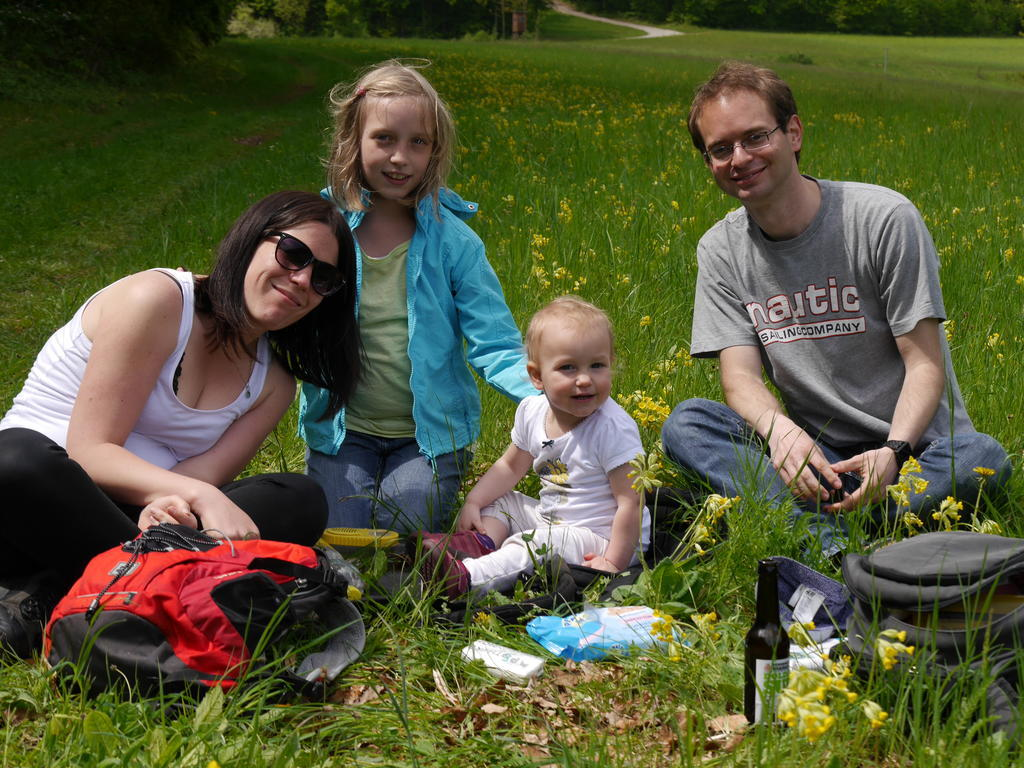
\includegraphics[width=\textwidth]{pic/US}
\end{figure}
\include{recipes/PumpkinSoup}
\include{recipes/CurlyKaleSoup}
\include{recipes/LinsenFenchelEintopf}
\include{recipes/TomatoeBredie}
\include{recipes/BroccoliNoodles}
\include{recipes/MushroomPolenta}
\include{recipes/ColeSlawWok}
\include{recipes/BrokkoliSuesskartoffelAuflauf}
\include{recipes/Cheese}
\include{recipes/AvocadoMouse}

\cleardoublepage
\section{Gerichte mit Fleisch}
\begin{figure}[h]
	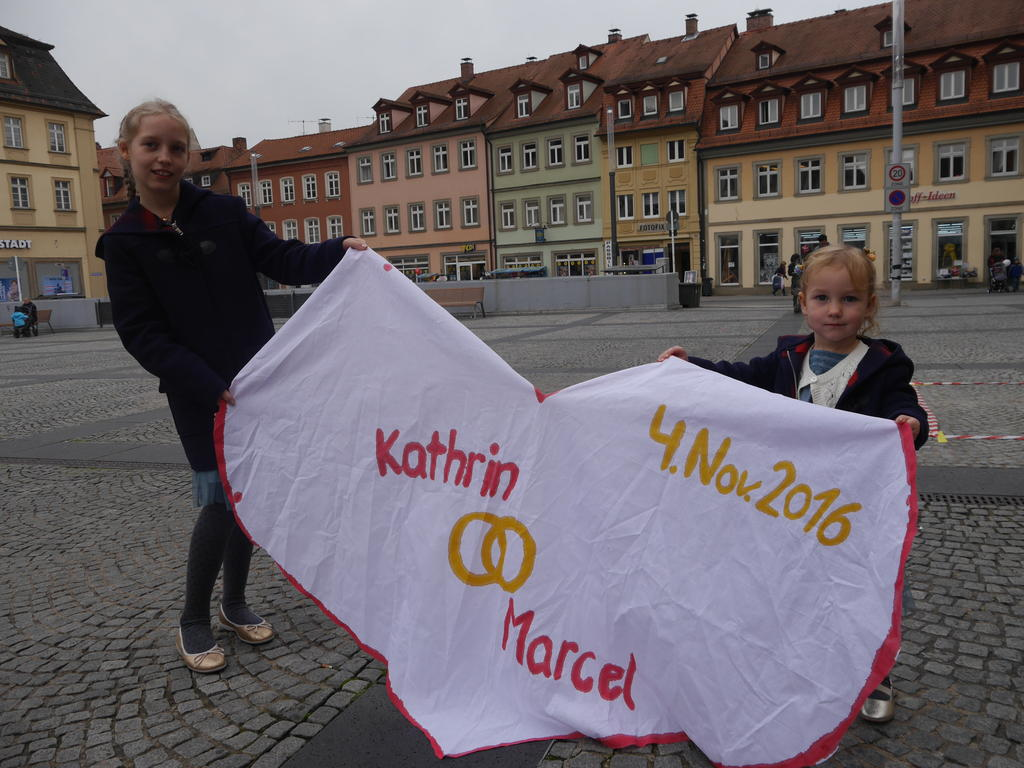
\includegraphics[width=\textwidth]{pic/fleisch.jpg}
\end{figure}
\begin{recipe}
[% 
    bakingtime={\unit[20]{min}},
    bakingtemperature={\protect\bakingtemperature{
        topbottomheat=\unit[100]{°C}}},
    portion = {\portion{2}},
    source = {Lieblingsrezept von Monika und Roland}
]
{Geschnetzeltes mit Reis}
   
    \ingredients{%
        3	& 	Schnitzel \\
	1	& 	Zwiebel \\
		1 &	Paprika \\
		&	Gemüsebrühe (instant) \\
		2 Hand & Reis\\
		&Gewürze\\
	optional & Käse\\
    }
    
    \preparation{%
    \newline
       \step Die Schnitzel in Streifen schneiden, in einer Pfanne anbraten und dabei nach Belieben würzen. Währenddessen als Beilage pro Person etwa eine Hand voll Reis mit der Brühe gar kochen.
       \step Zwiebel und Paprika würfeln, zum Geschnetzelten dazugeben und gut durchbraten.
       \step Rahmsoße dazugeben und alles gut durchmischen.
       \step Optional Käse darüber streuen und dann im Ofen ca. 20 min fertig braten.
    }
\end{recipe}
\begin{recipe}
[% 
    preparationtime = {\unit[15]{min}},
    bakingtime={\unit[20]{min}},
    portion = {\portion{4}},
    source = {Lieblingsrezept von Lars (original von chefkoch.de)}
]
{Schweizer Filet- oder Lendentopf}

    \ingredients{%
        400 g	& 	Schweinefilet(s) oder Lende \\
		2 Dosen & 	Champignons \\
		2 Becher    	&	süße Sahne \\
		3 Ecken	&	Schmelzkäse \\
		1	&	Zwiebel \\
		40 g	&	Käse (geriebener Emmentaler) \\
    }
    
    \preparation{%
    \newline
       \step Schweinefilet waschen und trocken tupfen. In etwas dickere Scheiben schneiden, würzen und kurz in einer beschichteten Pfanne mit wenig Öl von beiden Seiten anbraten.
       \step Gehackte Zwiebel glasig dünsten, anschließend Sahne, Champignons und Schmelzkäse dazu geben, etwas nachwürzen und aufkochen lassen. 
       \step Alles mit geriebenem Käse bestreuen und 20 Minuten bei ca. 150 °C ohne Deckel überbacken.    
    }
    
    \suggestion[Servierbeispiel]
    {%
        Dazu Rösti, Reis oder Pommes Frites reichen.
    }
    
    \hint{%
        Frische Champignons zusammen mit der Zwiebel anbraten und die Soße nach Belieben mit Weißwein verfeinern.\\
     Sahne und Schmelzkäse können für eine kalorienärmere Variante auch reduziert werden.
    }
    
\end{recipe}
% Complete recipe example
\begin{recipe}
[% 
    preparationtime = {\unit[45]{min}},
    portion = {\portion{4}},
    source = {Lieblingsrezept von Janina und Sebastian}
]
{Beegel mit Honigfrikadellen und Omelett}
    
    \graph
    {% pictures
        %small=pic/PumpkinSoup,     % small picture
       big=pic/Sebastian_Honigfrikadellen.jpg % big picture
    }
    
    %\introduction{%
     %   \blindtext
    %}
    
    \ingredients{%
        50 g & 	Joghurtsalatcreme\\
	50 g	& 	mittelscharfer Senf \\
		2 EL&	Ahornsirup \\
		80 g &	Cheddarkäse\\
		2 &Tomaten\\
		4 Stiele&Petersilie\\
		2 Scheiben&Toastbrot\\
		1 & Zwiebel\\
		1 Zweig & Rosmarin (klein)\\
		350 g & gemischtes Hack\\
		4 & Eier (Gr. M)\\
		2 EL & Honig\\
		2 EL & Milch\\
		1 EL & Butter\\
		1--2 EL & Öl\\
		4 & Bagels (à ca. 150 g)\\
	& Salz\\
	& Pfeffer\\
 }
    
    \preparation{%
    \newline
       \step Für den Dip Salatcreme, Senf und Ahornsirup verrühren. Mit Salz abschmecken. Käse grob raspeln. Tomaten waschen und in Scheiben schneiden. Petersilie waschen, trocken schütteln und hacken. 
       \step Für die Frikadellen Toast in kaltem Wasser einweichen. Zwiebel schälen und sehr fein würfeln. Rosmarin waschen, trocken tupfen, Nadeln abzupfen und fein hacken. Brot ausdrücken. Mit Hack, Zwiebel, Rosmarin, 1 Ei, Honig, 1 TL Salz und \unitfrac{1}{2} TL Pfeffer in einer Schüssel gut verkneten. 
\step Daraus 4 große, flache Frikadellen formen. 
\step 3 Eier und Milch verquirlen. Mit Salz und Pfeffer würzen. Butter in einer beschichteten Pfanne erhitzen. Eimasse darin bei schwacher Hitze stocken lassen, dabei mit einem Pfannenwender etwas zusammenschieben.  
\step  Herausnehmen, vierteln. Öl im Bratfett erhitzen. Frikadellen darin von jeder Seite ca. 4 Minuten braten.
\step Bagels waagerecht aufschneiden. Unterhälften mit etwas Dip bestreichen, jeweils mit 1 Frikadelle, 1 Stück Omelett und Tomaten belegen und mit Petersilie und Käse bestreuen. Darauf wieder etwas Dip geben, Deckel daraufsetzen.
    }
    
   \suggestion[Servierbeispiel]
   {%
Dazu passen Pommes Frites oder Süßkartoffel-Fries:\\
Kartoffeln schälen, gründlich waschen und in grobe Stifte schneiden. Kartoffeln, 3--4 EL Ahornsirup, 2 EL Öl und 1 TL Salz mischen. Auf ein mit Backpapier ausgelegtes Backblech verteilen. Im vorgeheizten Backofen (E-Herd: 200 °C / Umluft: 175 °C) 30--40 Minuten backen. Kartoffelsticks aus dem Ofen nehmen, eventuell mit groben Salz bestreuen, dazureichen.
    }
    
   % \suggestion{%
    %    \blindtext
   % }
    
%  \hint{%
 %              Auch lecker mit Kokosmilch anstelle von Sahne und Curry anstelle von
%Kreuzkümmel.\\
  %             Rote Bete im Schnellkochtopf etwa 7 Minuten (je nach Größe) garen und erst
%dann schälen und schneiden.
 %   }
    
\end{recipe}
\begin{recipe}
[% 
    preparationtime = {\unit[3 \unitfrac{1}{2}]{h}},
    bakingtime={\unit[2]{h}},
    portion = {\portion{6}},
    source = {Lieblingsrezept von Chris (original von chefkoch.de)}
]
{Eisbein gebraten}
    
    
    \ingredients{%
        1 \unitfrac{1}{2} kg	& 	Eisbein \\
		1 Zehe	& 	Knoblauch, gehackt \\
		1  &	mittelgroße Zwiebel, geviertelt \\
		1	&	Lorbeerblatt\\
		5 Körner	&	Piment \\
		5 Körner	&	Pfeffer \\
		\unitfrac{1}{2} TL & Kümmel \\
		2 TL & Salz\\
		 1 Liter & Wasser\\
    }
    
    \preparation{%
    \newline
     Den Backofen auf etwa 200° C vorheizen. 
       \step Ein großes Eisbein in einen Bräter legen, die Gewürze und den gehackten Knoblauch zugeben. Die Zwiebel schälen, vierteln, auch mit rein. Mit Wasser auffüllen, Salz nicht vergessen. 
       \step Nun den Bräter für 2 Stunden in den Backofen. Zwischendurch immer mal etwas Wasser nachgießen. Gegen Bratende soll aber mindestens noch 1/4l Flüssigkeit übrig sein.
       \step Wenn das Fleisch weich ist, vom Knochen entfernen. Vorsichtig, dass die Haut nicht abfällt. Die Fleischstücke mit der Schwarte nach oben nochmal in den Bräter und ohne Deckel etwa 20 min bräunen. 
    }
    
    \suggestion[Servierbeispiel]
    {%
       Passt zu Sauerkraut und Kartoffeln, aber auch zu Erbsenmus. 
	}
    
   \hint{%
        Wer das Fleisch gerne rosa möchte, sollte es 12 h vorher mit ein wenig Pökelsalz einreiben. 
    }
    \hint{Für einen noch würzigeren Sud können einige Babymöhren, \unitfrac{1}{2} Sellerieknolle, 4 TL Instantbrühe und etwas mehr Pfeffer, Lorbeerblätter und Nelken mitgebraten werden.}
    
\end{recipe}
\begin{recipe}
[% 
    portion = {\portion{4}},
    source = {Lieblingsrezept von Sina}
]
{Spiegeleier mit Bacon}
    
    \graph
    {% pictures
        small=pic/Sina_SpiegeleierMitBacon     % small picture
    }
     
    \ingredients{%
        8	& 	Eier (Größe L) \\
		16 Scheiben	& 	Bacon \\
		8 Scheiben &	Brot \\
			&	Butter \\
		& Salz\\
 & Pfeffer\\
    }
    
    \preparation{%
    \newline
       \step In einer Pfanne auf mittlerer Hitze den Bacon ohne Fettzugabe kross braten, dabei möglichst nur einmal wenden. Den Bacon aus der Pfanne nehmen und über der gleichen Pfanne die Eier vorsichtig aufschlagen, sodass beim Einlassen das Eigelb nicht verläuft. Die Eier vorsichtig würzen, Achtung der Bacon ist schon gut gesalzen, also nur wenig Salz verwenden, wenn nötig lieber nachsalzen. Während die Eier in der Pfanne sind, die Brote etwas mit wenig Butter bestreichen und mit dem Bacon belegen. Wenn das Eiweiß fest und nicht mehr durchsichtig ist, die Eier herausnehmen und auf den Bacon legen. \\Guten Appetit!
       
    }
       
   \hint{%
            Dieses Rezept ist vor allem geeignet zum Frühstück, oder wenn es mal schnell gehen muss ;)
    }
    
\end{recipe}
\begin{recipe}
[% 
     portion = {\portion{4}},
    source = {Lieblingsrezept von Sven (original Die Küchenschlacht)}
]
{Hausgemachte Tagliatelle mit Rinderfiletspitzen, Rucola und Tomaten}

    \ingredients{%
        600 g	& 	Rinderfiletspitzen \\
		200 g	& 	Rucola \\
		4 &	Schalotten \\
		2	&	Knoblauchzehen \\
		4 & Tomaten\\
2 & Zitronen\\
		 2 Bund & glatte Petersilie\\
		120 g & getrocknete Tomaten, eingelegt in Öl\\
		40 g& Pinienkerne\\
		100 g & Parmesankäse\\
		500 g & Mehl\\
		40 g & Hartweizengrieß\\
		4& große Eier\\
		& Zucker zum Abschmecken\\
		&Olivenöl zum Anbraten\\
					&	Butterschmalz zum Anbraten\\
			&	Pastagewürz zum Abschmecken \\
					&Schwarzer Pfeffer aus der Mühle\\
		& Salz aus der Mühle\\
    }
    
    \preparation{%
    \newline
       \step Das Mehl, den Hartweizengrieß und die Eier vermengen und zu einem Teig verarbeiten. Je nach Konsistenz
etwas Wasser zufügen. Anschließend den Teig ruhen lassen.
       \step Den Rucola waschen und die unteren Stiele abschneiden. Die Petersilienblätter waschen und vom Stängel
zupfen. Rucola und Petersilie zunächst in einer Schale zur Seite stellen.
       \step Die getrockneten Tomaten auf etwas Küchenpapier abtropfen lassen und in Streifen schneiden.
Die Pinienkerne in einer Pfanne ohne Öl anrösten. Eine Schalotte und einen Knoblauchzehe abziehen und
würfeln. Die Tomaten halbieren, vom Strunk befreien und fein hacken.
       \step Etwas Butterschmalz in einer weiteren Pfanne erhitzen und die Zwiebeln und den Knoblauch andünsten. Die
Pinienkerne, die Tomatenstreifen und Tomatenwürfel dazu geben. Die Zitrone waschen und halbieren.
Pinienkerne und Tomaten mit etwas
Zitronensaft und einer Prise Zucker abschmecken. Tomaten-
Pinienkernmischung auf niedriger Temperatur warm halten.
Anschließend den Parmesankäse reiben und zur Seite stellen.
     \step Für die Nudeln bereits einen Topf mit ausreichend Wasser aufsetzen und zum Kochen bringen. Den Nudelteig in
der Nudelmaschine zu Tagliatelle verarbeiten. Die Nudeln in dem kochenden Wasser mit etwas Salz gar kochen.
Anschließend abschütten.
 \step Die Rinderfiletspitzen waschen, trocken tupfen, mit Salz und Pfeffer würzen. Etwas Butterschmalz in einer Pfanne
erhitzen und das Rinderfilet kurz anbraten.
\step Den Rucola und die Petersilie kurz vor dem Anrichten in die Pfanne mit der Tomaten-Pinienkernmischung geben.
Nudeln und Filetspitzen dazugeben, alles schwenken und gut vermengen.
\step Die Tagliatelle mit den Filetspitzen, dem Rucola und den Tomaten auf einem Teller anrichten und mit dem
geriebenen Parmesan garnieren und servieren.
    }

\end{recipe}
\begin{recipe}
[% 
    preparationtime = {\unit[70]{min}},
    portion = {\portion{12}},
    source = {Lieblingsrezept von Petr}
]
{Borschtsch}

    
    \introduction{
Der Borschtsch ist weltweit bekannt. Es ist immer noch nicht klar, ob der Borschtsch ukrainisch oder russisch ist. Eigentlich ist es ja egal. Hauptsache, dass es schmeckt! \\
Die Prozesse des Fleischkochens und Vorbereitung der Gemüse lassen sich sehr gut parallelisieren. Den Borschtsch kann man auch vegetarisch machen, in dem das Fleisch auf dem Zubereitungsprozess eliminiert wird. \\
Die Anzahl der Zutaten bezieht sich auf 4-Liter-Topf.
    }
    
    \ingredients{%
    	1,0 kg & Rindfleisch (ein paar Knochen wären ganz gut für den Geschmack) \\
		500 g  & Kartoffeln \\
		300 g  & Gemüsekohl \\
		400 g  & rote Bete \\
		200 g  & Möhren \\
		200 g  & Zwiebeln \\
		3 El   & Tomatenpaste \\
		1 Tl   & Essig 6\% \\
		2–3    & Knoblauchzehen \\ 
		2–3    & Lorbeeren \\
	           & Salz \\
			   & Pfeffer \\
	           & Sonnenblumenöl \\
	           &\textbf{Dazu optional:}\\
	           &Schmand \\
&		Petersilie\\
&		Roggenbrot \\
&		Meerrettichaufstrich\\
&		Vodka\\
    }


    
    \preparation{%
    \newline
		\step Zunächst soll Rindfleisch 1.5 Stunden im Topf aufgekocht werden.
		\step Danach das Fleisch rausnehmen, würfeln und wieder in den Topf fügen.
		\step Zwiebel würfeln.
		\step Möhren auf der mittleren Oberfläche reiben.
		\step Gemüsekohl und rote Bete in Julienne schneiden.
		\step Rote Bete mit Sonnenblumenöl anbraten.
		\step Essig und Tomatenpaste hinzufügen und 5-7 Minuten dämpfen lassen.
		\step Zwiebel anbraten, nach ein paar Minuten Möhren hinzufügen. 
		\step Kartoffel würfeln. 
		\step In die kochende Brühe Kartoffel hinzufügen und anschließend salzen.
		\step Wenn die Brühe anfängt, wieder zu kochen, Gemüsekohl hinzufügen und 5 Minuten auf den mittleren Hitze lassen.
		\step Rote Bete hinzufügen und 10 Minuten aufkochen. 
		\step Möhren und Zwiebel hinzufügen. 
		\step Danach Lorbeeren hinzufügen und wenn nötig salzen und pfeffern. 
		\step Knoblauch pressen und dazu fügen. 
		\step Für ca. 20 Minuten ruhen lassen.     
    }
    
    \suggestion[Servieren]
    {%
        Der Borschtsch wird auf dem Teller mit Schmand und Petersilie serviert.
    }
    
    \hint{%
        Dazu passt ganz gut ein guter Shot Vodka und ein Stück Roggenbrot mit Meerrettich Aufstrich oben drauf!
    }
    
\end{recipe}
\begin{recipe}
[% 
    bakingtime={\unit[10]{min}},
    bakingtemperature={\protect\bakingtemperature{
        fanoven=\unit[160]{\textcelcius},
        topbottomheat=\unit[180]{°C},
     %   topheat=\unit[195]{°C},
       gasstove=Level 3}},
    portion = {\portion{4}},
    source = {Lieblingsrezept von Marie und Andreas}
]
{Kürbis-Apfel-Curry mit Entenbrust}
    
    \graph
    {% pictures
       big=pic/Marie_KuerbisApfelCurryMitEntenbrust  % big picture
    }
    
    \ingredients{%
        1	& 	Hokkaido-Kürbis (etwa 900g) \\
	4	& 	Schalotten \\
		1 &	rote Paprika \\
		1&	Knoblauchzehe \\
		1 & rote Chilischote\\
		4 EL &Öl\\
		&Salz\\
	2 & Sternanis\\
	1 TL & Currypaste (gelb)\\
	400 ml & Kokosmilch (Dose)\\
	1 Bund & Lauchzwiebeln\\
	4 & Äpfel (säuerlich, z.B. Boskop)\\
	2 & Entenbrustfilets (à 250-300g mit Haut, am besten Bio)\\
	2 TL & 5-Gewürze Pulver\\
	\unitfrac{1}{2}&Limette\\
	&frischer Pfeffer
    }
    
    \preparation{%
    \newline
       \step Kürbis und Paprika putzen, abspülen und in Würfel schneiden. Ingwer, Schalotten und Knoblauch
schälen. Ingwer und Knoblauch fein würfeln, Schalotten in Ringe schneiden. Chili abspülen und
fein hacken (mit Küchenhandschuhen arbeiten).
       \step Öl erhitzen, Kürbis portionsweise darin anbraten, salzen und herausnehmen. Ingwer,
Schalotten, Knoblauch, Chili und Sternanis in den Topf geben und andünsten.
       \step Paprika dazugeben und 1 Minute anbraten. Die Currypaste zufügen und ebenfalls 1 Minute
anbraten. Kokosmilch und Kürbisstücke zufügen. Zugedeckt 5--10 Minuten kochen. Lauchzwiebeln
putzen, abspülen, schräg in Ringe schneiden. Äpfel abspülen, vierteln, entkernen und in Spalten
schneiden.
       \step Backofen auf 180 Grad, Umluft 160 Grad, Gas Stufe 3 vorheizen.
       \step Entenbrust abspülen, trocknen, die Haut schräg bis in das Fettgewebe einritzen. Jede Entenbrust
auf der Hautseite mit je 1 TL 5-Gewürz-Pulver und 1⁄2 TL Salz einreiben. Das restliche Öl in einer
beschichteten Pfanne erhitzen, die Filets zuerst auf der Hautseite darin scharf anbraten, dann
wenden und noch 2 Minuten auf der Fleischseite braten. In Alufolie wickeln und im heißen Ofen
etwa 5-10 Minuten nachgaren lassen.
	\step Limettensaft auspressen. Die Apfelspalten in die Pfanne geben und im Entenbratfett goldbraun
anbraten. Zusammen mit den Lauchzwiebeln zum Curry geben, mit Salz, Pfeffer und Limettensaft
abschmecken.
	\step Entenbrustfilets aus der Folie nehmen und den aufgefangenen Fleischsaft aus der Folie zum
Curry geben. Fleisch in Scheiben schneiden, zusammen mit dem Curry servieren.
    }
    
   \suggestion[Servierbeispiel]
   {%
		Dazu Basmati-Reis und Koriander-Pesto!
    }
\end{recipe}
% Complete recipe example
\begin{recipe}
[% 
    preparationtime = {\unit[50]{min}},
    bakingtime={\unit[50]{min}},
    portion = {\portion{4}},
    source = {Ein weiteres Lieblingsrezept von Janina und Sebastian}
]
{Scharfe Erdnuss-Currysoße zu Schweinefilet}
    
    \graph
    {% pictures
        %small=pic/PumpkinSoup,     % small picture
       big=pic/Sebastian_Schweinefilet.jpg % big picture
    }
    
    %\introduction{%
     %   \blindtext
    %}
    
    \ingredients{%
        2 & 	Knoblauchzehen\\
	2	& 	Schalotten \\
		1 Stück&	Ingwer (ca. 20 g) \\
		1 &	Chilischote\\
		2 EL&geröstete Erdnüsse\\
		2&Schweinefilets (à ca. 350 g)\\
		3 EL&Öl\\
		2 EL & Tomatenmark\\
		3 EL & Erdnussbutter (Glas)\\
		2--3 TL & rote Currypaste \\
		400 ml & ungesüßte Kokosmilch\\
		3--4 EL & Sojasoße\\
		250 g & Zuckerschoten\\
		2--3 Stiele & Koriander\\
	& Salz\\
	& Pfeffer\\
	&brauner Zucker\\
 }
    
    \preparation{%
    \newline
       \step Für die Soße Knoblauch und 1 Schalotte schälen und fein würfeln. Ingwer schälen und fein reiben. Chili längs einschneiden, entkernen, waschen und hacken. Erdnüsse hacken.
       \step Ofen vorheizen (E-Herd: 150°C / Umluft: 125°C / Gas: s. Hersteller). Fleisch trocken tupfen. 2 EL Öl in einer großen Pfanne erhitzen und darin rundherum kräftig anbraten. Mit Salz und Pfeffer würzen. 
\step Auf ein Backblech legen und im heißen Ofen 10--12 Minuten braten. 
\step  Bratfett in der Pfanne erhitzen. Knoblauch, Schalottenwürfel, Ingwer und Chili darin andünsten, bis es duftet. Mit 1 TL braunem Zucker bestreuen und kurz karamellisieren. Tomatenmark, Erdnussbutter und Currypaste einrühren, kurz anschwitzen.
\step Kokosmilch, 100 ml Wasser und Sojasoße angießen. Aufkochen und 8--10 Minuten köcheln. Soße warm halten.
\step Die Zuckerschoten putzen, waschen und in Stücke schneiden. 1 Schalotte schälen und fein würfeln. 1 EL Öl erhitzen. Schalotte darin andünsten. Zuckerschoten und 2--3 EL Wasser zugeben und darin 2--3 Minuten garen. 
\step Koriander waschen, trocken schütteln und Blätter abzupfen. Fleisch herausnehmen und kurz ruhen lassen. Filet aufschneiden. Soße aufkochen. Alles anrichten und mit Koriander bestreuen.
    }
    
   \suggestion[Servierbeispiel]
   {%
Dazu schmeckt Reis.
    }
    
   % \suggestion{%
    %    \blindtext
   % }
    
%  \hint{%
 %              Auch lecker mit Kokosmilch anstelle von Sahne und Curry anstelle von
%Kreuzkümmel.\\
  %             Rote Bete im Schnellkochtopf etwa 7 Minuten (je nach Größe) garen und erst
%dann schälen und schneiden.
 %   }
    
\end{recipe}

\cleardoublepage
\section{Kuchen}
\begin{figure}[h]
	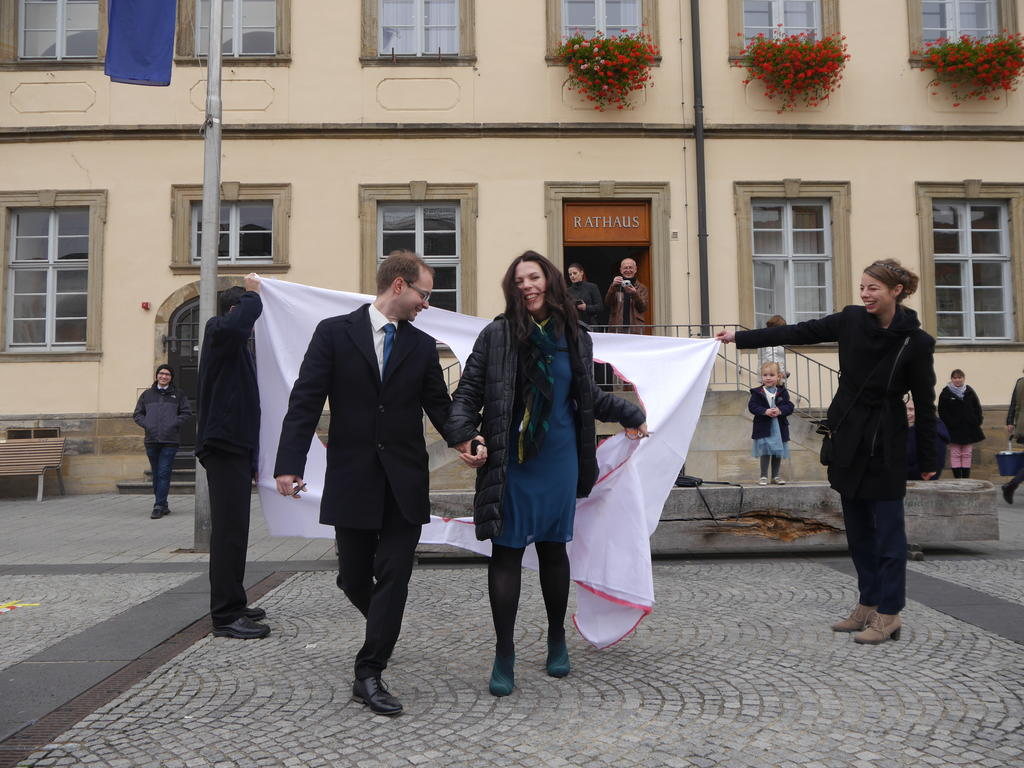
\includegraphics[width=\textwidth]{pic/kuchen.jpg}
\end{figure}

\begin{recipe}
[% 
    bakingtime={\unit[45]{min}},
    bakingtemperature={\protect\bakingtemperature{
        topbottomheat=\unit[160-170]{°C}}},
    portion = {\portion{2}},
    source = {Lieblingskuchen von Marie und Andreas}
]
{Sachertorte Originalrezept nach Carla Sacher}
   
   \ingredients{%
   		&\textit{1 dag = 10 g}\\
        28 dag	& 	Butter \\
	28 dag	& 	Zucker \\
		12&	Eier \\
		28 dag&	Schokolade \\
		22 dag & gesiebtes Mehl\\
		6 dag&Kakao\\
		&Marillenmarmelade\\
		&\textbf{Schokoladenglasur}\\
	75 dag& Schokolade\\
	3 dag& Kakao\\
	25 dag & Zucker oder Fondant\\
	ca. 125 ml& Wasser\\
 }
    
    \preparation{%
    \newline
       \step 28 dag Butter oder Rama mit 8 dag Zucker flaumig rühren.
       \step 12 Eidotter (bei kleinen Eiern mehr) unterrühren.
       \step 28 erweichte Schokolade – Achtung: nicht zu heiß, da sie sonst an Aroma
verliert – beigeben.
       \step 12 Eiklar zu Schnee schlagen, salzen, mit 20 dag Zucker zu festem Schnee
schlagen.
       \step 22 dag gesiebtes glattes Mehl und 6 dag Kakao unterrühren.
       \step Die Eisenringe mit Papier umwickeln und die Masse einfüllen.
       \step 45 Minuten bei 160-170 °C im Rohr backen.
       \step Erkalten lassen und aus den Ringen nehmen.
       \step In der Mitte durchschneiden, mit warmer Marillenmarmelade bestreichen und
zusammensetzen. Obere und äußere Seiten mit sehr heißer
Marillenmarmelade bestreichen.
\step 75 dag Schokolade zerkleinern.
\step 3 dag Kakao beigeben.
\step 25 dag Kristallzucker oder Fondant unterrühren.
\step 1/8 Liter Wasser (bei Bedarf etwas mehr) dazu leeren.
\step Köcheln lassen, bis kleine Fäden gezogen werden können.
\step Die Sachertorte mit der lippenwarmen Glasur übergießen.
    }
    
\end{recipe}

\begin{recipe}
[% 
    preparationtime = {\unit[30]{min}},
    bakingtime={\unit[80]{min}},
    bakingtemperature={\protect\bakingtemperature{
        fanoven=\unit[170]{\textcelcius}}},
    source = {Lieblingskuchen von Linus}
]
{Bierkuchen}
        
    
    \ingredients{%
        100g	& Butter \\	
		250g    & Zucker \\
		2		& Eier \\
		1 TL	& Zimt \\
		1 TL	& Nelken \\
		100g 	& Zitronat\\
		100g 	& Orangeat\\
		250g	& Sultaninen\\
		375g	& Mehl\\
		\unitfrac{1}{2} Seidla & Bier, nicht zu hopfig \\
		1 TL	& Natron\\
    }
    
    \preparation{%
    \newline
       \step Butten weich werden lassen, Natron im Bier aufl"osen und zusammen mit den anderen Zutaten gut verr"uhren. Nebenbei vom restlichen Bier trinken -- R"uhren ist nunmal anstrengend.
       \step Masse in eine gro\ss e, unter Umst"anden gefettete Kastenkuchenform einf"ullen.
       \step Backen. Dauert lange, aber man kann sich ja noch ein weiteres Bier aufmachen.
       \step Nach dem Backen ausk"uhlen lassen und mit Puderzucker bestreuen.
    }
    \suggestion{Es bietet sich an den Kuchen "uber Nacht stehen zu lassen, damit er sein Aroma optimal entfalten kann.}

    \hint{%
       Der Kuchen b"ackt zwar sehr lange, daf"ur ist er aber auch "uber eine Woche lang haltbar -- sofern er so "uberhaupt lange "uberlebt. 
    }
    
\end{recipe}
\begin{recipe}
[% 
    bakingtime={\unit[25]{min}},
    bakingtemperature={\protect\bakingtemperature{
        fanoven=\unit[160]{\textcelcius}}},
    source = {Lieblingskuchen von Marie und Andreas}
]
{Fantaschnitten mit Pfirsichschmand}
    
    \graph
    {% pictures
       small=pic/Marie_FantaschnittenMitPfirsichschmand % big picture
    }
    
    
    \ingredients{%
    &\textbf{Für den Teig:}\\
        4	& 	Eier (M) \\
	250 g	& 	Zucker \\
		1 Pck.&	Vanillinzucker \\
		125 ml&	Öl \\
		150 ml & Limonade (Fanta)\\
		250 g&Mehl\\
		3 TL&Backpulver\\
		&\textbf{Für den Belag:}\\
	2 Dosen& Pfirsich (Abtropgewicht 470 g)\\
	600 ml & Schlagsahne\\
	3 Pck. & Sahnesteif\\
	5 Pck. & Vanillinzucker\\
	500 g & Schmand\\
	& Zimt und Zucker zum Bestreuen\\    }
    
    \preparation{%
    \newline
       \step Für den Teig Eier, Zucker ud Vanillinzucker schaumig schlagen. Öl und Fanta unterrühren. Mehl und Backpulver mischen und unterrühren.
       \step Den Teig auf ein gefettetes Backblech streichen und in den Backofen geben. Im vorgeheizten Backofen bei 160 Grad (Heißluft) ca. 25 Minuten backen lassen.
       \step Den Kuchen auf dem Blech erkalten lassen.
       \step Für den Belag Pfirsiche abtropfen lassen und in kleine Stücke schneiden. Sahne mit Sahnesteif und 3 Päckchen Vanillinzucker steif schlagen. Schmand mit den restlichen 2 Päckchen Vanillinzucker verrühren. Pfirsichstücke unter den Schmand rühren und die Sahne unterheben.
       \step Die Masse gleichmäßig auf den Kuchen streichen und mit Zimtzucker bestreuen.
    }
    

   \hint{%
	   Anstelle von Pfirsichen können auch 2 Dosen Mandarinen verwendet werden.
   }
    
\end{recipe}
\begin{recipe}
[% 
    preparationtime = {\unit[15]{min}},
    bakingtime={\unit[17]{min}},
    bakingtemperature={\protect\bakingtemperature{
        fanoven=\unit[175]{\textcelcius}}},
    source = {Lieblingsmuffins von Marie und Andreas (original chefkoch.de)}
]
{Apfel-Muffins mit Rosinen und Nüssen}
    
    
    \ingredients{%
        2 \unitfrac{1}{2}	Tassen& 	Speisekleie (Haferkleie, keine Haferflocken)\\
	\unitfrac{1}{4} Tasse	& 	brauner Zucker \\
		\unitfrac{1}{4} TL&	Zimt \\
		1 EL&	Backpulver\\
		\unitfrac{1}{4} Tasse &Walnüsse oder Pecanüsse, gehackt\\
		\unitfrac{1}{4} Tasse&Rosinen\\
		1&mittelgroßer Apfel, fein geraspelt\\
	\unitfrac{3}{4} Tasse& Milch\\
	\unitfrac{3}{4} Tasse& Dicksaft (Apfeldicksaft)\\
	2 & kleiner Eier\\
	2 EL&Öl 
 }
    
    \preparation{%
    \newline
       \step Die trockenen Zutaten mit dem Apfel in einer Schüssel vermischen. Milch, Apfeldicksaft, Eier und Öl in einer anderen Schüssel oder im Mixer mischen. Zu den trockenen Zutaten geben und kurz vermengen.
       \step Ein Muffinblech einfetten oder mit Papierförmchen auslegen und den Teig einfüllen. 17 Minuten bei 175 Grad Umluft backen. Abkühlen lassen und genießen.
    }
    
  \hint{%
               Wenn man keinen Apfeldicksaft hat, kann auch eine halbe Tasse Apfelsaft verwendet werden, dann aber etwas mehr Zucker nehmen.\\
               Als Öl eignen sich besonder gut Walnussöl oder Rapsöl. Gut schmeckt auch Albaöl (Rapsöl mit Buttergeschmack).
    }
    
\end{recipe}

\end{otherlanguage}

\clearpage
~\thispagestyle{empty}
% Last page
\clearpage
\thispagestyle{empty}
~
\vfill
\begin{center}
\begin{tikzpicture}[scale=1.5]
\fill (0,0) -- (-0.2, 0.1) -- (-4, 0) -- (-0.2, -0.1) -- cycle;
\fill (0,0) -- (0.2, 0.1) -- (4, 0) -- (0.2, -0.1) -- cycle;
\fill (0,0) circle (0.1);
\end{tikzpicture}
\end{center}


    Eine hochzeitliche Rezeptesammlung -- Gerichte die wir G"aste lecker finden! Wir hoffen ihr findet die eine oder andere Anregung und denkt beim Kochen und Genießen an uns und das wundersch"one Fest.
    
    Wenn ihr mal ausgeschlafen habt könnt ihr unsere ganzen pull-requests unter \url{https://github.com/whatever4711/cookbook} annehmen.
\end{document} 